\chapter{Classificação de Recursos}

\begin{comment}
	\section{UbiquitOS}

O projeto UbiquitOS da Universidade de Brasília foi construído com foco na adaptabilidade de serviços~\cite{gomes2007} e possui o objetivo de prover serviços para o usuário de maneira transparente para usuário, ou seja, sem que usuário perceba a influência de computação. Nesse projeto foi desenvolvido um middleware que permite que os dispositivos possuam \emph{drivers} para seus recursos. Esses drivers são registrados e seus serviços podem ser acessados por diversas aplicações que necessitem destes serviços.

\subsection{DSOA - \emph{Device Service Oriented Architecture}}

A DSOA foi definida baseada na arquitetura SOA(\emph{Service Oriented Architecture}). A SOA possui diversas características que podem auxiliar ambientes inteligentes, proporciona a capacidade da reutilização de recursos de software. Entretanto, por ser uma apenas uma arquitetura genérica, não leva em consideração características e limitações de ambientes inteligentes, descrevendo apenas serviços em alto nível e não define, ainda, um modelo de comunicação.

Na DSOA destacam-se cinco conceitos básicos:

\begin{itemize}
	\item Ambiente Inteligente:
		É um ambiente composto por pelo menos dois dispositivos capacidade de computação e conectados por meio de uma rede de comunicação coloborativa com os usuários do ambiente. O provimento de serviços para o usuário vem da interação das aplicações deste ambiente dinâmico. Essa dinamicidade do ambiente ubíquo se dá pelo fato que os usuários entram, saem e se movimentam no ambiente, além disso, trazem consigo seus dispositivos. É importante ressaltar que um ambiente inteligente neste trabalho não tem seu significado mais popular de ambiente com inteligência artificial.
	\item Dispositivo:
		É um aparelho que possua capacidade de comunicação e que abrigar aplicações ou disponibilizar seus recursos do ambiente inteligente para que outras aplicações possam utilizar de seus serviços.
	\item Recurso:
		É um grupo de funcionalidades relacionadas que podem ser acessadas por meio de interfaces pré-definidas.
		\begin{itemize}
			\item Interface do Recurso:
				O recurso é a entidade básica de interação entre dispositivos, visto que é por meio dele que as funcionalidades presentes no ambiente poderão ser acessadas. Para que isso possa é acontecer, é necessário que seja definida uma interface de comunicação que seja conhecida pelas entidades presentes no \emph{smart space}. Essa interface é constituída por dois elementos:
				\begin{itemize}
					\item Identificador:
						Responsável por identificar unicamente um recurso entre diversos recursos presentes no ambiente.
					\item Conjunto de serviços:
						Conjunto de serviços que constituem o recurso e são disponibilizados por ele.
				\end{itemize}
		\end{itemize}
	\item Serviço:
		É a implementação de uma funcionalidade disponibilizada para o ambiente pelo reucurso e uma interface conhecida.
		\begin{itemize}
			\item Interface do Serviço:
			\begin{itemize}
				\item Recurso:
					Recurso do qual o serviço faz parte. Os serviços são encontrados a partir dos recursos.
				\item Identificador:
					Responsável por identificar unicamente um serviço dentro do recurso.
				\item Parâmetros:
					Parâmetros que serão passados para o serviços realizar a funcionalidade requisitada.
			\end{itemize}
		\end{itemize}
	\item Aplicações:
		São as responsáveis pela implementação da inteligência do ambiente. As aplicações executam nos dispositivos presentes no ambiente e, a partir de informações providas pelos recursos do amibente, podem realizar ações. Elas interagem com o usuário intermediando suas ações junto ao ambiente. Elas funcionam se relacionando com recursos para notificar o usuário da alteração de algum estado, ou aguardam a execução de algum comando por parte do usuário.
\end{itemize}

\subsection{\emph{uP - Ubiquitous Protocols}}

É um conjunto de protocolos criados para estabelecer um meio de interação entre serviços levando em consideração a arquitetura DSOA. Esses protocolos definem o canal de comunicação e a forma de interação entre entidades do ambiente. As mensagens são transmitidas no formato JSON (\emph{JavaScript Object Notation}), que utiliza a codificação UTF-8, que foi escolhido por ser um formato estruturado, leve e independente de plataforma. O JSON foi utilizado ante o XML, pois possui menor tamanho de mensagens e esse fator pode ser decisivo em um ambiente com diversos dipositivos com capacidades computacionais diferentes. Dessa forma a limitação dos dispositivos é minimizada e exclui a necessidade de uma rede para tratamento dessas mensagens.

Cada um dos conceitos apresentados na DSOA possuem uma representação no \emph{uP} com seus respectivos atributos:

\begin{itemize}
	\item Dispositivo(\emph{UpDevice}):
	
		Por meio dos seguintes atributos, é possível identificar unicamente o dispositivo no ambiente, e quais são as interfaces rede que o dispositivo possui para realizar alguma comunicação:
		\begin{itemize}
			\item \emph{``name''}: 
			
			Identificador do dispositivo;
			\item \emph{``networks''}: 

			Lista de interfaces de rede do dispositivo. Cada interface é composta pelo tipo de rede e endereço do dispositivo.
		\end{itemize}
	\item \emph{Driver}(\emph{UpDriver}): 

		Representa o conceito do Recurso definido na DSOA. Como um dispositivo pode ter várias instâncias de um recurso, cada instância é identificada unicamente dentro do dispositivo que contém este recurso. O \emph{driver} é composto por:
		\begin{itemize}
			\item \emph{``name''}:

				Identificador do recurso no ambiente;
			\item \emph{``services''}:
				
				Lista de serviços síncronos do recurso;
			\item \emph{``events''}:
				
				Lista de serviços assíncronos do recurso.
		\end{itemize}
	\item Serviço(\emph{UpService}): 

		Representa o conceito de mesmo nome definido na DSOA. Sua interface é composta pelos seguintes atributos:
		\begin{itemize}
			\item \emph{``name''}:

				Identificador do serviço disponível no recurso;
			\item \emph{``parameters''}:
				
				Lista de parâmetros necessários para que o serviço seja executado. Esses parâmetros podem ser de dois tipos:
				\begin{enumerate}
					\item Opcional (\emph{OPTIONAL});
					\item Obrigatório (\emph{MANDATORY}).
				\end{enumerate}
		\end{itemize}
\end{itemize}

\subsubsection{Tipo de mensagens}

Para que possa haver interação entre as entidades no ambiente, o \emph{uP} especifica quatro tipos de mensagens e, caso exista necessidade,  podem ser personalizadas:

\begin{itemize}
	\item \emph{Service Call}: 

		Mensagem síncrona do \emph{uP}. Seus parâmetros são definidos por meio de suas propriedades, podendo ser obrigatórias ou opcionais:
		\begin{itemize}
			\item Obrigatórias:
				\begin{itemize}
					\item \emph{\bf{type}}: 

						Representa o tipo da mensagem. No caso desta mensagem, seu valor será \emph{``SERVICE\underline{ }CALL\underline{ }REQUEST''};
					\item \emph{\bf{driver}}: 

						Recurso do serviço requisitado;
					\item \emph{\bf{service}}:

						Nome do serviço requisitado;
					\item \emph{\bf{parameters}}:

						Contém os parâmetros do serviço.
				\end{itemize}
			\item Opcionais:
				\begin{itemize}
					\item \emph{\bf{instanceId}}:

						Representa o identificador único da instância do \emph{driver} do serviço requisitado;
					\item \emph{\bf{serviceType}}:
						
						Representa a forma de transmissão de dados;
					\item \emph{\bf{channelIDs}}:

						Representa os identificadores dos canais criados para a comunicação;
					\item \emph{\bf{channelType}}:

						Representa o tipo da rede utilizada na comunicação.
				\end{itemize}
		\end{itemize}
	\item \emph{Service Response}: 

		Mensagem que carrega dados da resposta dada pela execução de um serviço chamado pelo \emph{Service Call}. Essa mensagem possui as seguintes propriedades:
		\begin{itemize}
			\item \emph{\bf{type}}: 

				Representa o tipo da mensagem. No caso desta mensagem, seu valor será \emph{``SERVICE\underline{ }CALL\underline{ }RESPONSE''};
			\item \emph{\bf{responseData}}: 

				Parâmetro opcional que contem os dados da resposta da execução do serviço.
		\end{itemize}
	\item \emph{Notify}: 

		Similar ao \emph{Service Response}, porém carrega dados de notificações de eventos, ou seja, respostas de uma requisição assíncrona de um serviço. Suas propriedades são:
		\begin{itemize}
			\item \emph{\bf{type}}: 

				Representa o tipo da mensagem. No caso desta mensagem, seu valor será \emph{``NOTIFY''};
			\item \emph{\bf{driver}}: 

				Recurso do serviço requisitado;
			\item \emph{\bf{instanceId}}: 

				Representa o identificador da instância onde ocorreu evento;
			\item \emph{\bf{parameters}}: 

				Parâmetro opcional com informações sobre o evento.
		\end{itemize}
	\item \emph{Encapsulated Message}: 

		Utilizada para permitir mensagens codificadas. Esse tipo de mensagem possui as seguintes propriedades:
		\begin{itemize}
			\item \emph{\bf{type}}: 

				Representa o tipo da mensagem. No caso desta mensagem, seu valor será \emph{``ENCAPSULATED\underline{ }MESSAGE''};
			\item \emph{\bf{securityType}}: 

				Identificador do tipo de codificação utilizada;
			\item \emph{\bf{innerMessage}}: 

				Mensagem codificada.
		\end{itemize}
\end{itemize}

\subsubsection{Protocolos}

Com o objetivo de disponibilizar as características de visibilidade, interação e efeito, foram criados mecanismos de acesso aos recursos. O \emph{uP} é dividido em protocolos básicos, que são utilizados para invocar serviços e protocolos complementares que completam suas  funcionalidas.

\begin{itemize}
	\item Protocolos Básicos: 

		São divididos em SCP (\emph{Service Call Protocol}) e EVP(\emph{Event Protocol}). O primeiro possui arquitetura provedor-consumidor, ou seja, o consumidor requisita um serviço e o provedor retorna esse serviço para ele de forma síncrona. No último, o consumidor se registra em um evento no provedor, que response informando que o registro foi realizado com sucesso, e na ocorrência do evento, o consumidor é notificado pelo provedor, demonstrando uma forma assíncrona de comunicação.
	\item Protocolos Complementares:

		Além da interação entre os serviços provida pelos protocolos básicos, o \emph{uP} tem mecanismos que permitem que as aplicações obtenham informações sobre quais são os serviços disponíveis no ambiente e informações a respeito deles. Os protocolos são divididos em um grupo de protocolos com informações sobre o dispositivo e um grupo de protocolos com informações sobre o ambiente. Esses grupos são mapeados em um \emph{driver} que definem sua interface de comunicação. São protocolos complementares:
	\begin{itemize}
		\item \emph{Device Driver}: 

			Responsável por disponibilizar informações a respeito do dispositivo. Possui os seguintes serviços:
			\begin{itemize}
				\item \emph{ListDrivers}: 

					Provê uma lista de instâncias dos drivers disponíveis do dispositivo. Possui dois parâmetros opcionais:
					\begin{itemize}
						\item \emph{\bf{serviceName}}: 

							Nome do serviço;
						\item \emph{\bf{driverName}}: 

							Identificador do recurso.
					\end{itemize}
				\item \emph{Handshake}: 

					Neste protocolo, dois dispositivos trocam informações entre-si. O dispositivo que invoca esse serviço passa como parâmetro um objeto do tipo \emph{device} e recebe como retorno informações sobre o dispositivo que recebeu a chamada;
				\item \emph{Goodbye}: 

					Responsável por retirar o dispositivo da lista de dispositivos presentes no ambiente;
				\item \emph{Authenticate}: 

					Estabelece um contexto de segurança entre dois dispositivos por meio de um prévio compartilhamento de chaves.
			\end{itemize}
		\item \emph{Register Driver}: 

			Responsável por disponibilizar informações que um dispositivo possui sobre o ambiente.
			\begin{itemize}
				\item \emph{ListDrivers}: 

					Provê uma lista de instâncias dos drivers disponíveis no ambiente, geralmente de dispositivos vizinhos. Possui três parâmetros opcionais:
					\begin{itemize}
						\item \emph{\bf{serviceName}}: 

							Nome do serviço;
						\item \emph{\bf{driverName}}: 

							Identificador do recurso;
						\item \emph{\bf{device}}: 
							
							Nome do dispositivo que contém o recurso.
					\end{itemize}
				\item \emph{Publish}: 

					Responsável pela publicação de uma instância de um driver a ser disponibilizada no ambiente.
				\item \emph{UnPublish}: 

					Responsável por retirar as informações sobre uma instância de um driver.
			\end{itemize}
	\end{itemize}
\end{itemize}
\end{comment}

Ambientes de computação ubíqua são compostos por recursos de rede que proveem diversas funcionalidades usualmente abstraídas por protocolos de comunicação intedependentes de plataformas. Um importante desafio para tais ambientes é o desenvolvimento de técnicas de descoberta de recursos que permitam que aplicativos clientes localizem serviços e dispositivos. Tais técnicas devem atingir três objetivos principais~\cite{balazinska2002ins/twine}:

\begin{enumerate}
	\item Lidar com descrições de recursos sofisticados e padrões de consulta;
	\item Lidar com o dinamismo no ambiente operacional, incluindo mudanças no estado dos recursos e conexões;
	\item Ser escalável para um grande número de recursos.
\end{enumerate}

Neste sentido, destaca-se a importância de uma classificação de recursos que possibilite uma melhor gerência dos diversos recursos presentes no \emph{smart space}. Tal classificação livrará o usuário de tarefas e configurações tediosas e redundantes, evitando quaisquer custos administrativos de forma a facilitar a interação entre diferentes aparelhos, contribuindo para a adaptabilidade de serviços.

A fim de ilustrar a vantagem em se empregar a classificação de recursos em técnicas de descoberta de recursos, considere o seguinte exemplo:

Um usuário presente em um \emph{smart space} que não possui uma classificação de recursos necessita de uma tela para projetar a apresentação do seu trabalho de graduação que está armazenada em seu celular. Existem três recursos de tela disponíveis: \emph{Wide40InchesScreen}, \emph{Nice27InchesScreen} e \emph{Small14InchesScreen}. Como fazer para selecionar uma das telas? Caberia ao usuário buscar por cada um dos recursos disponíveis, pois para o ambiente tais telas não possuem relação. Outro problema ocorreria com a saída do ambiente de um dos recursos que estivessem sendo utilizados pelo usuário. O que fazer para supri-lo? A única alternativa seria entregar outro recurso idêntico ao anterior, de forma a garantir a existência dos serviços necessários para a sua correta execução. Com a implementação da classificação de recursos, todos estes problemas seriam facilmente sanados, com tudo ocorrendo de forma transparente ao usuário. Ao se necessitar de uma tela, realizaria-se uma única busca por \emph{Screen}, obtendo como resultado todas as telas disponíveis. Se um recurso tornar-se indisponível, não só recursos idênticos poderiam substituir o anterior, mas também todos aqueles que possuírem os serviços necessários para a correta execução da tarefa em andamento. A imagem~\ref{fig:arvoreDeEquivalencia} apresenta um exemplo da estrutura dessa classificação, em que \emph{WideScreen} e \emph{LetterBoxScreen} são uma especialização de \emph{Screen}.

\begin{figure}[ht]
	\center
	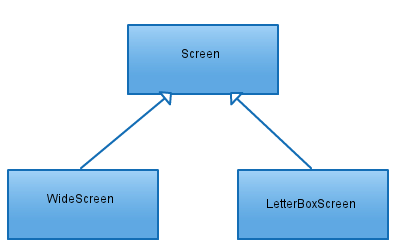
\includegraphics[scale=0.8]{imagens/screenTree}
	\caption{Classificação de recursos.}
	\label{fig:arvoreDeEquivalencia}
\end{figure}

\begin{comment}
Como descrito anteriormente, o \emph{uOS} tem como foco a adaptabilidade de serviços, em que cada serviço pertence a um determinado recurso. Este, por sua vez, possui um identificador (ou nome), que o representa unicamente entre os demais. Esta abordagem, apesar de funcional, é deficiente, pois cada \emph{driver} é visto de maneira isolada dos outros.

Imagine, por exemplo, o caso em que uma aplicação necessita de um serviço de \emph{snapshot} presente em um recurso de câmera. Suponha também que, dentre os diversos dispositivos registrados na base do \emph{middleware}, existam quatro que possuam o serviço desejado:

\begin{figure}[ht]
	\center
	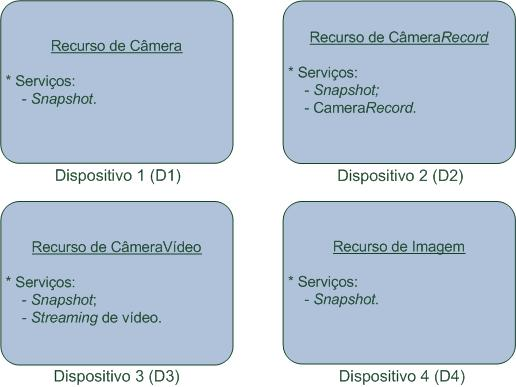
\includegraphics[scale=0.8]{imagens/recursos}
	\caption{Exemplos de recursos presentes no \emph{smart space}.}
	\label{fig:recursos}
\end{figure}

Dito isto, cabe ao \emph{uOS} determinar qual recurso será selecionado à aplicação requisitante. Entretanto, considere que o recurso preferencial (D1) esteja indisponível. Neste caso, o sistema deverá repassar um outro recurso que seja equivalente ao primeiro. Entende-se por equivalente todo recurso que:

\begin{itemize}
	\item Possua o mesmo identificador;
	\item Possua serviços equivalentes. Neste caso, tais serviços devem possuir o mesmo retorno e a mesma assinatura, ou seja, mesmos nome, quantidade, tipo e ordem de parâmetros.
\end{itemize}

Repare que D2, D3 e D4 também possuem o serviço de \emph{snapshot}, mas enquanto D4, por se tratar de um recurso de natureza completamente distinta, não poderia ser utilizado de forma alguma pela aplicação solicitante, D2 e D3 poderiam sem perda de funcionalidade. Contudo, de acordo com a definição acima, isso não é possível, visto que D1, D2 e D3 são recursos diferentes e, portanto, não são equivalentes. Como dito inicialmente, essa deficiência é causada justamente pelo fato de cada \emph{driver} ser visto de forma isolada e não-relacionada pelo \emph{middleware}. Este trabalho tem como um dos objetivos solucionar este problema.
\end{comment}

\section{Formas de classificação}

Definiu-se duas formas principais de se realizar uma classificação de recursos:

\begin{enumerate}
	\item Fixa: conjunto fixo de classificações não-relacionadas e, portanto, mais simples de serem definidas.

	\item Relacionada: conjunto de classificações básicas relacionadas com suas especializações. Passível de organização hierárquica, de forma que cada especialização possua automaticamente em sua definição todos os serviços presentes em sua classe superior e, obrigatoriamente, pelo menos um serviço adicional.
\end{enumerate}

\subsection{Formas de representação}

Para tornar possível o processo de classificação de recursos, faz-se necessária uma maneira de representar de forma hierárquica todas as possíveis classes existentes no \emph{smart space}. Abaixo, seguem algumas das estratégias mais utilizadas atualmente:

\begin{itemize}
	\item Hierarquia de classes: amplamente utilizada na programação orientada à objetos por meio da herança, seja ela simples ou circular;

	\item JSON~\cite{json}: linguagem de marcação auto-descritiva independente de plataforma e de baixo custo computacional. É estruturada e pode formar uma estrutura em árvore. Não necessita de pré-processamento para se tornar compreensível~\cite{comparativojson}. Utiliza UTF-8 como codificação~\cite{utf8};
	
	\item Ontologia: descrição formal, em um determinado domínio, de conceitos que descrevem atributos, características, restrições e possuem propriedades. Assim como na hierarquia de classes, também permite herança simples ou circular;

	\item XML (\emph{Extensible Markup Language})~\cite{xml}: linguagem de marcação auto-descritiva independente de plataforma desenvolvida para estruturar, armazenar e transportar dados. Utiliza \emph{tags} (que devem ser previamente definidas pelo usuário) para realizar suas marcações e pode ser estendida de forma a criar uma estrutura em árvore. Não necessita de pré-processamento computacional para se tornar compreensível. Como desvantagem, apresenta o fato de repetir grande quantidade de informação, o que pode ser prejudicial à velocidade de comunicação entre dois sistemas.
\end{itemize}

\section{Padrões}
%Apresentar os padrões. Focar nas classificações feitas por eles, pontos fortes e fracos.

A seguir, seguem cinco dos principais protocolos e/ou padrões pesquisados que fazem uso de uma classificação de recursos e utilizam as estratégias supracitadas para representar sua hierarquia de recursos: UPnP, IEEE 1451, DLNA, USB, \emph{Bluetooth} e DDL.

\subsection{UPnP}
O \emph{Universal Plug and Play Protocol} (UPnP) é um protocolo para conectividade entre aplicações inteligentes utilizado em computadores e dispositivos, \emph{wireless} em geral. Foi definido com o objetivo de facilitar a conectividade entre dispositivos em diferentes ambientes, como casas, pequenas empresas ou espaços públicos~\cite{upnpArch}. Não necessita de configurações e fornece uma rede invisível com descoberta automática de dispositivos de diferentes fabricantes e diversas categorias.

Seu nome ``Universal'' advém da não utilização de \emph{drivers} para cada dispositivo. Para tal, utiliza protocolos bem conhecidos como IP, TCP, UDP e HTTP, além do formato XML, utilizado no armazenamento de informações como fabricante, lista de dispositivos embarcados, descrição dos serviços com lista de comandos e ações com parâmetros e argumentos, URL's de controle, eventos e apresentação.

Quando um novo aparelho adentra na rede, ele recebe um IP via DHCP ou gera um IP para si (no caso de redes não-gerenciadas), publica seus serviços, disponibiliza uma URL e conhece os serviços de outros dispositivos. A \emph{UPnP Device Architecture}(UDA) divide os dispositivos em duas categorias principais: controlados, também chamados de ``dispositivos'' e pontos de controle~\cite{upnpArch}, estabelecendo uma arquitetura cliente-servidor onde pontos de controle acessam os serviços disponibilizados pelos dispositivos. Após a entrada desse novo aparelho na rede, os pontos de controle ainda não têm muita informação sobre o dispositivo, então os pontos de controle interessados solicitam a descrição do dispositivo por meio da URL disponibilizada anteriormente.

O UPnP estabelece uma classificação composta por um conjunto de tipos pré-determinados. Quando um fabricante deseja produzir um novo dispositivo, este deve se adequar a estes tipos ou estabelecer um novo tipo próprio. Uma característica interessante dessas classificações é que elas podem ser implementadas por dispositivos com pouca capacidade de computação, embora também possam ser utilizadas por dispositivos mais robustos como computadores, ou seja, são independentes de plataforma. Os tipos presentes no UPnP são:

\begin{itemize}
\item Áudio/Vídeo:

	Essa categoria possui duas principais sub-classificações que foram sendo atualizadas com o surgimento de novas tecnologias: 
	\begin{itemize}
		\item \emph{Media Server}:

			Define um dispositivo genérico que provê conteúdo de áudio e/ou vídeo, como CD e DVD \emph{players}, cameras, rádios, televisões e \emph{set-top boxes}. Embora, seja utilizado por dispositivos com diferentes capacidades de processamento, diferentes conteúdos e em diferentes formatos, o \emph{Media Server} expõe o conteúdo disponível de forma uniforme e consistente por meio de um Diretório de Conteúdo.

		\item \emph{Media Renderer}:

			Define um dispositivo genérico capaz de renderizar conteúdos de áudio e/ou vídeo como MP3 \emph{players} e televisões. Dependendo da implementação de um \emph{Media Renderer}, pode-se utilizar os recursos de auto-falante de uma televisão para consumir um serviço de música de um \emph{Media Server}.
	\end{itemize}
\item Gerenciamento de Dispositivos:

	Essa categoria foi criada para adicionar operações gerenciais à qualquer dispositivo UPnP. Essa gerência inclui funções para configuração de serviços e do próprio dispositivo, diagnóstico e correção de problemas além de gerência do \emph{firmware} e dos \emph{softwares} do dispositivo.

\item Automação Residencial:

	O UPnP define quatro tipos de dispositivos de automação residencial:
	\begin{itemize}
		\item Cortina de Proteção Solar:

			Provê uma sombra por meio de uma cortina. Seu controle pode ser manual, automático ou desabilitado. Sua especificação não contempla configurações a respeito da automação da cortina ou proteções.
		\item Câmera Digital de Segurança:

			Provê controle básico sobre a configuração da câmera, contendo serviços de fotos e vídeos.
		\item Aquecimento, Ventilação e Ar-Condicionado:
			
			Esse dispositivo conta com auxílio de sensores de temperatura e possui a capacidade de saber ou controlar a temperatura do ambiente por meio de ventiladores e ar-condicionados.
		\item Controles de Luz:
			
			São divididos em Luz binária, que representa uma lâmpada ou qualquer dispositivo emissor de luz que possa somente estar apagado ou aceso, e em Luz cuja intensidade pode ser alterada, 
	\end{itemize}

\item Rede:

	Nessa categoria se enquadram dispositivos relacionados com uma rede, seja um \emph{gateway} ou um ponto de acesso local.
	\begin{itemize}
		\item \emph{Gateway} de Internet:
			
			Essa classificação define um dispositivo de interconexão entre uma rede residencial local (LAN) e a \emph{Wide Area Network} (WAN), provendo conectividade com a internet.
			\begin{itemize}
				\item Dispositivo de Conexão WAN: É um dispositivo virtual definido tendo o \emph{Gateway} de Internet como raiz. Funciona como um contêiner para um \emph{link} ou serviços de conexão em uma interface WAN. 
				\item Dispositivo WAN: É um dispositivo virtual definido tendo o \emph{gateway} de internet como raiz. Cada dispositivo WAN é uma instância virtual de uma interface WAN no \emph{gateway} de internet. Múltiplas interfaces físicas WAN para clientes UPnP, existirão distintas instâncias deste dispositivo.
			\end{itemize}

		\item Ponto de acesso WLAN(\emph{Wireless Local Area Network}):
			
			Esse dispositivo implementa os padrões IEEE 802.11 (a,b,g) sem fio para prover uma infraestrutura de rede para casas e pequenas empresas. Essa definição não inclui uso dos pontos de acesso como \emph{hotspots} ou redes de grandes empreendimentos. O ponto de acesso age como uma ponte \emph{Ethernet} que permite ligações de múltiplos nós com a LAN.
	\end{itemize}

\item Impressora:

	Define um dispositivo com capacidade de impressão. Essa especificação não abrange dispositivos que possuem funções de FAX ou \emph{Scanner}, que possui uma especificação própria.

\item Acesso Remoto:

	Essa categoria comporta dispositivos que possam servir tanto comoé dividida entre dois dispositivos:
	\begin{itemize}
		\item Agente de Descoberta de Acesso Remoto:

			Possui a função de prover a capacidade de sincronizar a informação sobre a descoberta UPnP entre duas redes remotas.
		
		\item Servidor de Acesso Remoto:
		
			Permite que pontos de controle configurem Servidores de Acesso Remoto.

	\end{itemize}

\item Interface Remota:

	Classifica dispositivos entre servidores e clientes de uma interface remota com o usuário.

\item \emph{Scanner}:

	Representa um dispositivo de \emph{Scanner} com \emph{feeder} opcional. Esse dispositivo possui os serviços de digitalização via \emph{feeder} ou \emph{flatbed} e um serviço para configuração com o painel frontal do dispositivo. Essa categoria não contempla funcionalidades de Fax ou cópias.

\item Telefonia:
	
	Categoria para aparelhos que se relacionam com algum serviço de telefonia, tanto como consumidor quanto como con provedor.
	\begin{itemize}
		\item Servidor de Telefonia:

			Permite que pontos de controle gerenciem chamadas telefônicas, mensagens e presença por meio de outros dispositivos UPnP. 

		\item Cliente de Telefonia:
		
			Permite que pontos de controle possam gerenciar mídias por meio de um de um servidor de telefonia.
				
	\end{itemize}

\item Básico:

	A definição de dispositivos básicos provêem um mecanismo para produtos que não se enquadram em uma classificação adequada do UPnP, possam utilizá-lo. Por esse motivo, essa especificação não possui nenhum serviço definido, mas pode ser utilizada como dispositivo raiz para outras categorias já definidas.
\end{itemize}

A partir de uma classificação padrão, os fabricantes podem, por exemplo, estender e especializar determinada definição adicionando novos serviços, o que sugere a formação de uma hierarquia de dispositivos por meio de arquivos XML. O UPnP, portanto, utiliza uma classificação dispositivos relacionada, o que facilita a criação de novos tipos de dispositivos a partir da classficação base agregando novos serviços. Essa classificação extendida, entretanto, deve passar por um processo de certificação. Um ponto forte nas classificações é o fato de já incluírem a especificação dos serviços que os dispositivos proveem.

\subsection{IEEE 1451}
O IEEE 1451 se divide em uma família de padrões que foram criados com os objetivos de permitir a capacidade de comunicação entre transdutores(sensores e atuadores) de forma \emph{plug-and-play} por meio de redes com ou sem fio, facilitar a criação de transdutores com inteligência embarcada, simplificar a configuração e manutenção de sistemas, prover comunicação entre transdutores legados, e por fim, habilitar a implementação de transdutores inteligentes e com uso mínimo de memória~\cite{ieee1451journal}.

Um dos padrões da família, o IEEE 1451.1, define um modelo de informação para \emph{Network Capable Application Processors} (NCAP) que foi estabelecido para especificar um modelo de objetos comum e interfaces de componentes da rede de transdutores. Dessa forma, foi desenvolvido um \emph{framework} orientado a objetos que pode ser estendido para facilitar o desenvolvimento de aplicações. Este modelo foi definido da seguinte forma: Um modelo de dados que especifica a forma e o tipo de comunicação, tanto local quanto remota, por meio das interfaces de objetos 1451.1, um modelo de objetos que especifica tipos de componentes de software usados para definir e implementar sistemas e, por fim, modelos de comunicação que definem a sintaxe e semântica das interfaces de software entre redes de comunicação e objetos de aplicação~\cite{ieeeOO1451}~\cite{ieee1451monitoring}.


O padrão ~\cite{ieee1451standard} especifica cada classe no modelo definindo as interfaces da classe(por meio de assinaturas e operações) e o comportamento da classe (via texto ou máquinas de estado). Abaixo temos a hierarquia de classes definida pelo padrão:

\lstset{caption={Classes de Dispositivos do Padrão IEEE 1451},label=dispositivos1451}
\begin{lstlisting}[frame=single]
Root
	Entity
		Block
			NCAP BLOCK
			Function Block
			Base Transducer Block
			Transducer Block
				Dot2 Transducer Block
				Dot3 Transducer Block
				Dot4 Transducer Block
		Component
			Parameter
				Parameter With Update
					Physical Parameter
						Scalar Parameter
							Scalar Series Parameter
						Vector Parameter
							Vector Series Parameter
				Time Parameter
			Action
			File
				Partitioned File
			Component Group
		Service
			Base Port
				Base Client Port
					Client Port
					Asynchronous Client Port
				Base Publisher Port
					Publisher Port
					Self Identifying Publisher Port
					Event Generator Publisher Port
			Subscriber Port
			Mutex Service
			Condition Variable Service
\end{lstlisting}

\begin{comment}
\begin{tabbing}
\textit{Root} \= \\
\> \textit{Entity} \= \\
\> \> \textit{Block} \= \\
\> \> \> NCAP BLOCK \\
\> \> \> \textit{Function Block} \\
\> \> \> \textit{Base Transducer Block} \\
\> \> \> \textit{Transducer} \= \textit{Block} \\
\> \> \> \> Dot2 Transducer Block \\
\> \> \> \> Dot3 Transducer Block \\
\> \> \> \> Dot4 \= Transducer Block \\
\> \> \textit{Component} \\
\> \> \> Parameter \\
\> \> \> \> Parameter With Update \\
\> \> \> \> \> \= \textit{Physical Parameter} \\
\> \> \> \> \> \> Scalar \= Parameter \\
\> \> \> \> \> \> \> Scalar Series Parameter \\
\> \> \> \> \> \> Vector Parameter \\
\> \> \> \> \> \> \> Vector Series Parameter \\
\> \> \> \> Time Parameter \\
\> \> \> Action \\
\> \> \> File \\
\> \> \> \> Partitioned File \\
\> \> \> Component Group \\
\> \> \textit{Service} \\
\> \> \> \textit{Base Port} \\
\> \> \> \> \textit{Base Client Port} \\
\> \> \> \> \> Client Port \\
\> \> \> \> \> Asynchronous Client Port \\
\> \> \> \> \textit{Base Publisher Port} \\
\> \> \> \> \> Publisher Port \\
\> \> \> \> \> Self Identifying Publisher Port \\
\> \> \> \> \> \> \> Event Generator Publisher Port \\
\> \> \> Subscriber Port \\
\> \> \> Mutex Service \\
\> \> \> Condition Variable Service \\
\end{tabbing}
\end{comment}

É possível observar 3 tipos principais de objetos IEEE 1451.1:

\begin{itemize}
	\item\emph{Block}:

	Especializada em três classes:
		\begin{itemize}
			\item\emph{NCAPBlock}:

				Provê interfaces para comunicações de rede e configurações do sistema. Cada NCAP é modelado para possuir ao menos um processo de software. Cada processo de processo de software possuirá exatamente um \emph{NCAPBlock}.
			\item\emph{BaseTransducerBlock}:

				Provê interfaces entre transdutores e funções.
			\item\emph{FunctionBlock}:

				Provê encapsulamento de funções específicas.
		\end{itemize}
	
	\item\emph{Component}:
	
		Fornecem:
		\begin{itemize}
			\item Informações estruturadas: medidas e arquivos.
			\item Coleções de objetos relacionados com a aplicação.
			\item Ações com estados onde a ação é executada após um período de tempo.
		\end{itemize}
	\item\emph{Service}:
	
		Suportam:
		\begin{itemize}
			\item Comunicação entre objetos de diferentes NCAPs.
			\item Sincronização do sistema.
		\end{itemize}
\end{itemize}

Há ainda as classes não-IEEE 1451.1, que não estão representadas na hierarquia acima e possuem restrições de aplicabilidade na arquitetura IEEE 1451. Este padrão possui a limitação de ter sido criado para sensores e atuadores.



\subsection{DLNA}

A \emph{Digital Living Network Alliance} (DLNA) é uma organização composta pelas principais empresas de eletrônicos de consumo, computação e dispositivos móveis, tais como: Microsoft, Sony, Nokia, Samsung, Cisco entre outros. Foi fundada em 2003 e tem como objetivo fornecer orientações para permitir a interoperabilidade entre dispositivos para completar a convergência da indústria digital, levando, dessa forma, inovação, simplicidade e valor aos consumidores~\cite{dlnaoverview}. Tem como visão facilitar a criação, o gerenciamento e o compartilhamento de conteúdo digital (fotos, músicas e vídeos) entre os dispositivos pertencentes à mesma rede~\cite{dlnahdvideostreaming}. Deve permitir, por exemplo~\cite{dlnaoverview}:

\begin{itemize}
	\item facilmente adquirir, armazenar e acessar música digital a partir de praticamente qualquer lugar da casa;
	\item facilmente gerenciar, visualizar, imprimir e compartilhar fotos digitais;
	\item transportar seu conteúdo favorito a partir de qualquer lugar, mesmo que as pontas envolvidas estejam em movimento;
	\item aproveitar a gravação e reprodução de conteúdo distribuído e multi-usuário.
\end{itemize}

Suas diretrizes destacam casos de uso construídos para redes domésticas, funções adicionais que aumentam a experiência do compartilhamento de conteúdo e doze classes de dispositivos espalhados na categoria ``Rede Doméstica e Dispositivos Móveis''. A classificação de um dispositivo é feita de tal forma que um único aparelho multifuncional pode possuir diversas categorias diferentes~\cite{dlnahdvideostreaming, dlnaclasses}:

\begin{itemize}
	\item \emph{Home Network Devices} (HND)
	\begin{itemize}
		\item \emph{Digital Media Server} (DMS): 

		Esses dispositivos armazenam e disponibilizam conteúdo para \emph{Digital Media Players} (DMP) e \emph{Digital Media Renderes} que estão conectados na rede. Alguns servidores de mídia podem ainda proteger o conteúdo do usuário uma vez que ele tenha sido armazenado. Exemplo: PCs e dispositivos de armazenamento via rede(NAS);
		\item \emph{Digital Media Player} (DMP): 

		Esses dispositivos encontram conteúdo disponibilizados pelos servidores de mídia (DMS) e provêem a capacidade de reprodução e renderização de mídia. Exemplos: TVs, aparelhos de som, \emph{home theaters}, monitores sem fio e vídeo games;
		\item \emph{Digital Media Renderer} (DMR): 

		Esses dispositivos tocam conteúdos recebidos do controlador digital de mídia (DMC) que, por sua vez, irá encontrar conteúdo do servidor de mídia digital (DMS). Exemplos: TVs, receptores de áudio ou vídeo, projetores de vídeo e alto-falantes remotos para música;
		\item \emph{Digital Media Controller} (DMC): 

		Esses dispositivos encontram conteúdo em servidores de mídia digital (DMS) e o tocam em renderizadores de mídia digital (DMR). Exemplos: \emph{tablets}, câmeras digitais com Wi-Fi e PDAs;
		\item \emph{Digital Media Printer} (DMPr): 

		Esses dispositivos provêem serviços de impressão para a rede residencial DLNA. Geralmente, tocadores de mídia digital (DMP) e controladores de mídia digital (DMC) com a capacidade de impressão podem utilizar o DMPr para impressão. Exemplo: impressoras de foto e multifuncionais conectadas na rede DLNA.
	\end{itemize}
	\item \emph{Mobile Handheld Devices} (MHD)
	\begin{itemize}
		\item \emph{Mobile Digital Media Server} (M-DMS): 

		Esses dispositivos sem fio armazenam conteúdo e o tornam disponível para tocadores de mídia digital que tenham acesso à rede sem fio ou com fio (M-DMP), renderizadores de mídia digital (DMR) e impressoras de mídia digital (DMPr). Exemplo: telefones portáteis e tocadores portáteis de música;
		\item \emph{Mobile Digital Media Player} (M-DMP): 

		Esses dispositivos sem fio encontram e tocam conteúdo de um servidor de mídia digital (DMS) ou servidor móvel de mídia digital (M-DMS). Exemplo: telefones portáteis, \emph{tablets} projetados para visualização de conteúdo multimídia;
		\item \emph{Mobile Digital Media Uploader} (M-DMU): 

		Esses dispositivos sem fio enviam conteúdo para um servidor digital de mídia (DMS) ou para um servidor móvel de mídia digital (M-DMS). Exemplo: câmeras digitais, e telefones portáteis;
		\item \emph{Mobile Digital Media Downloader} (M-DMD): 

		Esses dispositivos sem fio encontram e armazenam conteúdo de um servidor de mídia digital (DMS) ou de um servidor móvel de mídia digital (M-DMS). Exemplo: tocadores de música e telefones portáteis;
		\item \emph{Mobile Digital Media Controller} (M-DMC): 

		Esses dispositivos encontram conteúdo em um servidor digital de mídia(DMS) ou em um servidor móvel de mídia digital (M-DMS) e o envia para renderizadores de mídia digital(DMR). Exemplo: telefones portáteis e PDAs.
	\end{itemize}
	\item \emph{Home Infrastructure Devices} (HID)
	\begin{itemize}
		\item \emph{Mobile Network Connectivity Function} (M-NCF): 

		Esses dispositivos provêem uma ligação entre a conectividade de rede de dispositivos móveis portáteis e conectividade de rede residencial;
		\item \emph{Media Interoperability Unit} (MIU): 

		Esses dispositivos provêem transformação de conteúdo entre formatos de mídia necessários para uma rede residencial ou para dispositivos móveis portáteis.
	\end{itemize}
\end{itemize}

\begin{table}
	\caption{Camadas padrões DLNA~\cite{dlnahdvideostreaming}.}
	\begin{center}
		\begin{tabular}{rp{5cm}p{5cm}}
		\hline
		\textbf{Camada} & \textbf{Função definida} & \textbf{Padrões}				\\
		\hline
		Transmissão Protegida & Como um conteúdo comercial está protegido em uma rede doméstica. & DTCP/IP \\
		\hline
		Formatos de Mídia & Como um conteúdo de mídia está codificado e identificado para interoperabilidade. & MPEG2, MPEG4, AVC/H.264, LPCM, MP3, AAC LC, JPEG, XHTML-Print- \\
		\hline
		Transporte de Mídia & Como um conteúdo de mídia é transferido. & HTTP, Quality of Service \\
		\hline
		Gerência de Mídia & Como um conteúdo de mídia é identificado, gerenciado e distribuído. & UPnP AV 1.0, UPnP Print Enhanced 1.0 \\
		\hline
		Descoberta e Controle & Como dispositivos se descobrem e se controlam um ao outro. & UPnP Device Architecture 1.0 \\
		\hline
		Redes IP & Como dispositivos com e sem fio fisicamente se conectam e se comunicam. & IPv4 Protocol Suite \\
		\hline
		Conectividade & Com qual rede os dispositivos se conectam e se comunicam& Wired: Ethernet 802.3, MoCAWireless: Wi-Fi 802.11, Wi-Fi Protected Setup \\
		\hline
		\end{tabular}
	\end{center}
	\label{tab:camadaspadroes_dlna}
\end{table}

\begin{comment}
\begin{table}
	\caption{Classes DLNA~\cite{}.}
	\begin{center}
		\begin{tabular}{llll}
		\hline
		\textbf{Classe} & \textbf{Categoria} & \textbf{Descrição} & \textbf{Exemplo}						\\
		\hline
		\hline
		Mobile Network Connectivity Function (M-NCF) & \multirow{2}{*}{Home Infrastructure Devices} &  & \\
		\hline
		Media Interoperability Unit (MIU) & &  & \\
		\hline
		\end{tabular}
	\end{center}
	\label{tab:classes_dlna}
\end{table}
\end{comment}

Considere como exemplo a Figura~\ref{fig:traditionalProccess}, em que uma pessoa deseja compartilhar um pequeno vídeo com seus amigos a partir de seu celular. A fim de exibir esse vídeo em sua TV widescreen na sua sala de estar, ela necessita, primeiramente, enviá-lo para seu próprio email. Em seguida, deve ligar seu PC, fazer o download do vídeo e salvá-lo em um \emph{pendrive} ou cartão de memória. Posteriormente, deve ligá-lo na TV ou em um receptor digital e, então, utilizar a interface do dispositivo para localizar o vídeo e exibi-lo~\cite{dlnahdvideostreaming}, tornando-se, dessa forma, um processo tedioso e demora que os consumidores raramente farão.

Além de interromper a conversa, esse tipo de processo de transferência de conteúdo exige tempo e atenção em excesso do usuário, mesmo quando ocorre sem problemas. Como resultado, a partilha informal de vídeo em múltiplas telas não é vista, muitas vezes, como uma opção razoável~\cite{dlnahdvideostreaming}.

\begin{figure}[ht]
	\center
	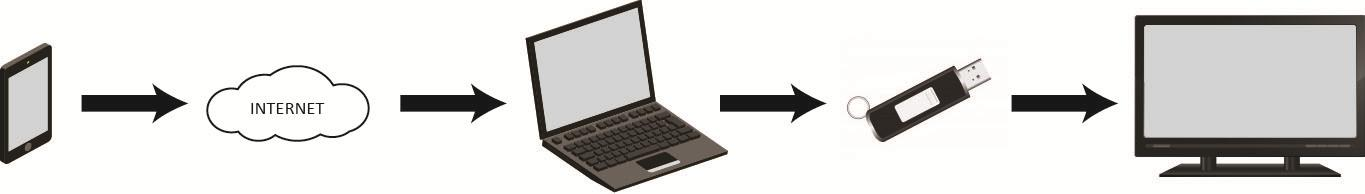
\includegraphics[scale=0.3]{imagens/dlna1}
	\caption{Processo de exibição de um vídeo, que está armazenado em um celular, em uma TV.}
	\label{fig:traditionalProccess}
\end{figure}

Este é o objetivo das organizações com compõem a DLNA: oferecer aos seus consumidores a partilha contínua e sem esforço de conteúdo digital, permitindo o envio de fotos ou vídeos para a TV em uma única etapa (Figura~\ref{fig:dlnaProccess}). O consumidor pode até mesmo congelar o vídeo usando um ``controle remoto'' do menu no telefone, bem como \emph{fast-forward} e reproduzir o vídeo~\cite{dlnahdvideostreaming}.

\begin{figure}[ht]
	\center
	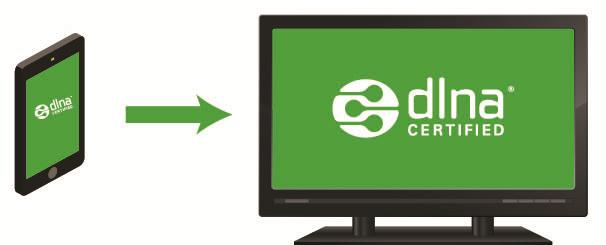
\includegraphics[scale=0.3]{imagens/dlna2}
	\caption{Envio de conteúdo de digital para TV em uma única etapa.}
	\label{fig:dlnaProccess}
\end{figure}

Desta forma, o DLNA pode ser visto como um aglomerado de camadas e seus respectivos padrões abertos (Tabela~\ref{tab:camadaspadroes_dlna}) que definem como uma rede residencial interage em todos os seus níveis, ou seja, além de definir como os diferentes padrões irão interoperar e como os dados serão tratados em cada nível, ele também reduz o número de padrões que um dispositivo deve suportar.

\begin{comment}
\begin{itemize}
       \item Enviar: 

       Transferir vídeos ou imagens capturadas em uma câmera digital ou celular para um computador;
       \item Empurrar: 

       Exibir vídeos ou imagens capturadas em uma câmera digital ou celular diretamente em uma TV sem intermédio de um computador;
       \item Localizar e Reproduzir ou ``Reproduzir em...'': 

       Utiliza um celular para localizar uma música ou vídeo armazenados em um computador, unidade de disco externa ou um dispositivo \emph{Network-Attached Storage} (NAS) e transferi-lo, via \emph{stream} ou não, para reprodução;
       \item Puxar e imprimir ou ``Imprimir em...'': 

       Visualizar na TV uma foto armazenada em um servidor de mídia e imprimi-la utilizando uma impressora em rede.
\end{itemize}

\begin{table}
	\caption{Exemplos de casos de uso~\cite{dlnahdvideostreaming}.}
	\begin{center}
		\begin{tabular}{rl}
		\hline
		\textbf{Casos de Uso} & \textbf{Exemplo}																\\
		\hline
		Enviar & Transferir vídeos ou imagens capturadas em uma câmera digital ou celular para um computador.	\\
		\hline
		Empurrar & Exibir vídeos ou imagens capturadas em uma câmera digital ou celular diretamente em uma TV sem intermédio de um computador. \\
		\hline
		Localizar e Reproduzir ou ``Reproduzir em...'' & Utiliza um celular para localizar uma música ou vídeo armazenados em um computador, unidade de disco externa ou um dispositivo \emph{Network-Attached Storage} (NAS) e transferi-lo, via \emph{stream} ou não, para reprodução. \\
		\hline
		Puxar e imprimir ou ``Imprimir em...'' & Visualizar na TV uma foto armazenada em um servidor de mídia e imprimi-la utilizando uma impressora em rede. \\
		\hline
		\end{tabular}
	\end{center}
	\label{tab:casosdeuso_dlna}
\end{table}
\end{comment}


\subsection{USB}

O \emph{Universal Serial Bus} (USB) é uma arquitetura de comunicação que adiciona a uma máquina hospedeira a capacidade de se interconectar a uma variedade de dispositivos. Seu intuito é sanar três das principais dificuldades enfrentadas à época de sua criação~\cite{usbspec}:

\begin{itemize}
	\item Integrar as plataformas das industrias da informática e comunicação. Para tal, a troca de informações entre esses dispositivos deveria acontecer de forma ubíqua e barata;
	\item Facilitar a reconfiguração de dispositivos de um computador, tais como teclados, mouses e \emph{joysticks};
	\item Integrar todas as interfaces existentes à época em um única que pudesse ser utilizada pela maior quantidade possível de dispositivos: telefone, fax, \emph{modem}, adaptadores, secretárias eletrônicas, \emph{scanners}, PDA's, teclados, \emph{mouses}, etc.
\end{itemize}

De acordo com sua especificação, suas máquinas hospedeiras devem:

\begin{itemize}
	\item Fornecer energia aos seus periféricos;
	\item Suportar todas as velocidades definidas (\emph{SuperSpeed}, \emph{Low Speed}, \emph{Full Speed} e \emph{High SuperSpeed});
	\item Suportar todos os tipos de fluxo de dados definidos (controle, massa, interrupção e síncrono).
\end{itemize}

Entende-se por máquina hospedeira qualquer dispositivo possuidor dos recursos necessários para realizar esta função. Por exemplo, conectar uma câmera à uma impressora faz sentido, enquanto que conectar um GPS à mesma impressora, não. Assim sendo, cada máquina hospedeira não necessita se comportar exatamente como um computador, mas apenas servir como hospedeiro a certos dispositivos convenientes.

Atualmente sua velocidade de comunicação varia entre 1.5 ou 12 megabits por segundo (MB/s) e seu protocolo permite configurar dispositivos durante a fase de inicialização ou quando eles são plugados em tempo de execução~\cite{hid}, deixando toda parte onerosa desse processo a cargo do hospedeiro. Tais dispositivos são divididos em várias classes e subclasses diferentes, cada qual definindo um comportamento e protocolos comuns para dispositivos que oferecem funções similares.

Um mesmo dispositivo USB pode pertencer a uma ou múltiplas classes. Por exemplo, um celular pode utilizar atributos da classe HID, Áudio e Comunicação. A partir dessas divisões será possível estabelecer uma hierarquia, que será usada no processo de classificação dos dispositivos presentes no \emph{smart space}. A seguir seguem as classes definidas por este padrão~\cite{usbclasscodes}:

\begin{itemize}
	\item \emph{Audio}: 

	Destina-se a todos os dispositivos ou funções embutidos em aparelhos que são usados para manipular áudio, voz e quaisquer funcionalidades relacionadas. Isso inclui tanto dados de áudio (analógico e digital) quanto a capacidade de diretamente controlar tal ambiente por meio de controles de volume e tom. Não inclui a funcionalidade para operar mecanismos de transporte que estão relacionados com a reprodução de dados de áudio, tais como mecanismos de transporte de fita ou controles de unidade de CD-ROM~\cite{usbaudioclass}. Exemplos de tais dispositivos incluem \emph{headsets}, \emph{headphones} e \emph{microphones}~\cite{usbbasicaudioclass}.
	\item \emph{Communications and CDC Control}: 

	Há três classes que compõem a definição de dispositivos de comunicação: a Classe de Comunicação do Dispositivo, a Classe de Interface de Comunicação e a Classe de Interface de Dados. A primeira é uma definição de nível do dispositivo e é utilizada pelo hospedeiro para identificar corretamente um dispositivo de comunicação que pode apresentar diferentes tipos de interfaces. A segunda define um mecanismo de propósito geral que pode ser utilizado para habilitar todos os tipos de serviços de comunicação sobre o Universal Serial Bus (USB). A última define um mecanismo de propósito geral para permitir a transferência em massa quando os dados não atendem aos requisitos para qualquer outra classe~\cite{usbcommunicationclass}.	Exemplos de tais dispositivos incluem:
	\begin{itemize}
		\item Telecomunicações: 

		Modems analógicos, adaptadores de terminais ISDN, telefones digitais e telefones analógicos;
		\item Dispositivos de rede: 

		Modems ADSL, modems à cabo, adaptadores/hubs \emph{Ethernet} 10BASE-T e \emph{Ethernet} cross-over cabos.
	\end{itemize}
	\item HID (\emph{Human Interface Device}): 

	Destina-se primordialmente aos dispositivos que são usados por humanos para controlar e operacionalizar quaisquer tipos de sistemas computacionais~\cite{hid}. Mais específicamente, possui as seguintes particularidades:
	\begin{itemize}
		\item Deve ser tão compacto quanto possível para evitar desperdício de espaço no dispositivo;
		\item Permitir a aplicação de software para evitar informação desconhecida;
		\item Ser extensível e robusto;
		\item Suportar hierarquias e coleções;
		\item Ser autodescritivo para permitir aplicações de software genéricos.
	\end{itemize}

	Exemplos de tais dispositivos incluem: teclados e dispositivos apontadores, painéis de controle, controles que podem ser encontrados em dispositivos como telefones, controles remotos, jogos ou dispositivos de simulação e aparelhos que não necessitam de interação humana mas que fornecem dados de forma similar aos dipositivos da classe HID.
	\item \emph{Physical}: 

	É vista como uma extensão da classe HID para dispostivos que requerem resposta física em ``tempo real''. Seu foco principal está em dispositivos táteis e na implementação de sistemas com resposta à força. Contúdo, não há exigência de que os membros desta classe gerem esse tipo de efeito~\cite{usbphysicalclass}. Exemplos de tais dispositivos incluem: \emph{joysticks} e plataformas de movimento.
	\item \emph{Image}: 

	Destina-se aos dispositivos de captura de imagem~\cite{usbimageclass}. Exemplos de tais dispositivos incluem: câmeras digitais e aparelhos similares.
	\item \emph{Printer}: 

	Destina-se aos dispositivos de impressão. Estes, anteriormente, eram interfaceados por meio das seguintes tecnologias~\cite{usbprintclass}:
	\begin{itemize}
		\item Porta paralela unidirecional;
		\item Porta paralela bi-direcional;
		\item Porta serial;
		\item Porta SCSI;
		\item \emph{Ethernet} / LAN.
	\end{itemize}

	Atualmente existem outras interfaces mais sofisticadas, mas essas são as mais comuns. O USB oferece uma capacidade de processamento muito maior que a porta serial e é comparável em velocidade à porta paralela.
	\item \emph{Mass Storage}: 

	Destina-se aos dispositivos de armazenamento em massa, ou seja, todo aparelho que possa ler ou gravar dados digitais em algum sistema de armazenamento.	Exemplos de tais dispositivos incluem: pendrives, discos de estado sólido com memória flash não volátil e HD's.
	\item \emph{Hub}: 
	\item \emph{Smart Card}: 

	Destina-se aos dispositivos compostos por cartões de circuitos integrados~\cite{usbsmartcard}. Exemplos de tais dispositivos incluem: cartões de crédito, CPF's digitais, etc.
	\item \emph{Content Security}: 

	Destina-se primordialmente em proteger e controlar a distribuição de conteúdo digital. Especifica um conjunto comum de requisições de transporte de dados e descritores necessários para apoiar os vários métodos de segurança de conteúdo~\cite{usbcontentsecurityclass}.
	\item \emph{Video}: 

	Destina-se a todos os dispositivos ou funções que compõem outros aparelhos utilizados para manipular vídeos~\cite{usbvideoclass}. Exemplos de tais dispositivos incluem: \emph{webcams}, filmadoras digitais, conversores analógicos de vídeo, sintonizadores de televisão analógica e digital e imagens de câmeras que suportam \emph{streaming} de vídeo.
	\item \emph{Personal Healthcare}: 

	Destina-se em permitir a interoperabilidade entre aparelhos da saúde pessoal e hospedeiros USB, o que permite uma maior variedade de casos de uso para ambos os dispositivos e hospedeiros~\cite{usbhealthcareclass}. Exemplos de tais dispositivos incluem: medidores de glicose e oxímetros de pulso.
	\item \emph{Diagnostic Device}:

	Destina-se aos dispositivos que diagnosticam outros dispositivos.
	\item \emph{Wireless Controller}: 

	Destina-se aos dispositivos controladores \emph{wireless}. Exemplos de tais dispositivos incluem: aparelhos \emph{bluetooth} e via rádio.
	\item \emph{Miscellaneous}:

	Destina-se à dispositivos diversos.
	\item \emph{Application Specific}:

	Destina-se aos dispositivos que estejam em conformidade com as especificações da várias classes USB. Define um conjunto utilizável de subclasses e protocolos.
	\item \emph{Vendor Specific}:

	Destina-se à utilização por parte dos fornecedores, que podem usá-la como bem entenderem.
\end{itemize}

\subsection{\emph{Bluetooth}}

Destina-se a substituir os cabos de conexão de dispositivos fixos e/ou portáteis mantendo altos níveis de segurança. Sua força fundamental está na capacidade de lidar simultaneamente com dados e transmissão de voz, o que fornece aos usuários uma variedade de soluções inovadoras, tais como fones de ouvido \emph{hands-free} para chamadas de voz, impressão, fax, sincronização com PCs e telefones celulares, entre outros~\cite{bluetoothoverview}.

É uma tecnologia de comunicação de curto alcance. Suas principais características são a robustez, a baixa potência e o baixo custo. Sua especificação define uma estrutura uniforme para que uma ampla gama de dispositivos possam se conectar e se comunicar uns com os outros~\cite{bluetoothoverview}.

Sua estrutura e aceitação global permitem que qualquer dispositivo \emph{bluetooth} ativado possa se conectar a outros dispositivos \emph{bluetooth} situados em sua proximidade. Para isso, cada dispositivo deve ser capaz de interpretar certos perfis, ou seja, definições de aplicações possíveis que especificam comportamentos gerais. No mínimo, cada perfil contém informações sobre os seguines tópicos~\cite{bluetoothprofiles}:

\begin{itemize}
	\item Dependências em outros perfis;
	\item Formatos de interface de usuário sugeridos;
	\item Partes específicas da pilha de protocolos \emph{bluetooth} utilizadas pelo perfil. Para executar sua tarefa, cada perfil utiliza opções específicas e parâmetros em cada camada da pilha e isso pode incluir, se for o caso, um esboço do registro de serviço exigido.
\end{itemize}

Seguem abaixo os perfis atualmente disponíveis~\cite{bluetoothprofiles}:

\begin{itemize}
	\item \emph{Advanced Audio Distribution Profile} (A2DP): 

	Define como um áudio estéreo pode ser transmitido de uma fonte de mídia para um dispositivo de armazenamento.

	Exemplos de tais dispositivos incluem: fones de ouvido, alto-falantes e adaptadores estéreos e reprodutores de MP3~\cite{bluetoothprofilesA2DP}.
	\item \emph{Audio/Video Remote Control Profile} (AVRCP): 

	Destina-se em fornecer uma interface padrão para controlar TV's, equipamentos de áudio estéreo ou outros dispositivos de áudio e vídeo. Permite que um único controle remoto (ou outro dispositivo) controle todos os equipamentos de áudio e vídeo que o usúario tenha acesso.

	Exemplos de tais dispositivos incluem: PC's, PDA's, celulares, controles remotos, fones de ouvido, reprodutores e gravadores de áudio e vídeo, monitores, TV's, sintonizadores e amplificadores~\cite{bluetoothprofilesAVRCP}.
	\item \emph{Basic Imaging Profile} (BIP): 

	Define como um dispositivo de imagem pode ser controlado remotamente, como um dispositivo de imagem pode imprimir e como um dispositivo de imagem pode transferir imagens para um dispositivo de armazenamento.

	Exemplos de tais dispositivos incluem: câmeras digitais, PC's, celulares, impressoras e PDA's~\cite{bluetoothprofilesBIP}.
	\item \emph{Basic Printing Profile} (BPP): 

	Permite que os dispositivos enviem texto, emails, \emph{v-cards}, imagens ou outras informações para impressoras com base em trabalhos de impressão.
	
	Exemplos de tais dispositivos incluem: impressoras, PC's, celulares e PDA's~\cite{bluetoothprofilesBPP}.
	\item \emph{Common ISDN Access Profile} (CIP): 

	Define como uma sinalização de uma Rede Digital de Serviços Integrados (ISDN, em inglês) pode ser transferida através de uma conexão \emph{bluetooth}.

	Exemplos de tais dispositivos incluem: \emph{laptops}, pontos de acesso, PC's e celulares~\cite{bluetoothprofilesCIP}.
	\item \emph{Cordless Telephony Profile} (CTP): 

	Define como um telefone sem fio pode ser implementado sobre um \emph{link} \emph{bluetooth}.

	Exemplos de tais dispositivos incluem: \emph{laptops}, PC's, telefones sem fios, celulares e PDA's~\cite{bluetoothprofilesCTP}.
	\item \emph{Dial-Up Network Profile} (DUN): 

	Fornece um padrão para acessar a internet e outros serviços \emph{dial-up} via \emph{bluetooth}.

	Exemplos de tais dispositivos incluem: \emph{laptops}, PC's, celulares, PDA's e modems~\cite{bluetoothprofilesDUN}.
	\item \emph{Fax Profile} (FAX): 

	Define como um dispositivo de FAX pode ser usado por um dispositivo de terminal.

	Exemplos de tais dispositivos incluem: \emph{laptops}, PC's, celulares, PDA's e modems~\cite{bluetoothprofilesFAX}.
	\item \emph{File Transfer Profile} (FTP): 

	Define como as pastas e os arquivos em um dispositivo servidor podem ser visitados por um dispositivo cliente.

	Exemplos de tais dispositivos incluem: \emph{laptops}, PC's, celulares e PDA's~\cite{bluetoothprofilesFTP}.
	\item \emph{General Audio/Video Distribution Profile} (GAVDP): 

	Fornece a base para o A2DP e o VDP, que são a base dos sistemas de distribuição projetados para fluxos de vídeo e áudio usando a tecnologia \emph{bluetooth}.

	Exemplos de tais dispositivos incluem: reprodutores de música, fones de ouvido e alto-falantes estéreos, \emph{laptops}, PC's, celulares e PDA's~\cite{bluetoothprofilesGAVDP}.
	\item \emph{Generic Object Profile} (GOEP): 

	Utilizado para transferir um objeto de um dispositivo para outro.

	Exemplos de tais dispositivos incluem: \emph{laptops}, PC's, celulares, PDA's e visualizadores de mídia~\cite{bluetoothprofilesGOEP}.
	\item \emph{Hands-Free Profile} (HFP): 

	Descreve como um dispositivo de \emph{gateway} pode ser usado para fazer e receber chamadas para um dispositivo \emph{hands-free}.

	Exemplos de tais dispositivos incluem: carros, kits automotivos, sistemas GPS, fones de ouvido, celulares e PDA's~\cite{bluetoothprofilesHFP}.
	\item \emph{Hard Copy Cable Replacement Profile} (HCRP): 

	Define como uma impressão baseada em driver é realizada através de uma conexão \emph{bluetooth}.

	Exemplos de tais dispositivos incluem: impressoras, PC's e \emph{laptops}~\cite{bluetoothprofilesHCRP}.
	\item \emph{Headset Profile} (HSP): 

	Descreve como um fone de ouvido deve se comunicar com um dispositivo habilitado para \emph{bluetooth}.

	Exemplos de tais dispositivos incluem: fones de ouvido, celulares, PDA's, PC's e \emph{laptops}~\cite{bluetoothprofilesHSP}.
	\item \emph{Human Interface Device Profile} (HID): 

	Define os protocolos, procedimentos e recursos a serem utilizados por teclados \emph{bluetooth}, \emph{mouses}, dispositivos de jogos e apontandores e dispositivos de monitoramento remoto.

	Exemplos de tais dispositivos incluem: teclados, \emph{mouses}, dispositivos de jogos, \emph{tablets}, PC's, \emph{laptops}, celulares e PDA's~\cite{bluetoothprofilesHID}.
	\item \emph{Intercom Profile} (ICP): 

	Define como dois celulares \emph{bluetooth} em uma mesma rede podem se comunicar diretamente sem usar o telefone público ou rede celular.

	Exemplos de tais dispositivos incluem: celulares, PC's e \emph{laptops}~\cite{bluetoothprofilesICP}.
	\item \emph{Object Push Profile} (OPP): 

	Define as regras dos servidores e clientes \emph{push}.

	Exemplos de tais dispositivos incluem: celulares, PC's e \emph{laptops}~\cite{bluetoothprofilesOPP}.
	\item \emph{Personal Area Networking Profile} (PAN): 

	Descreve como dois ou mais dispositivos \emph{bluetooth} podem formar uma rede ad-hoc e como este mecanismo pode ser usado para acessar uma rede remota através de um ponto de acesso à rede.

	Exemplos de tais dispositivos incluem: celulares, PC's e \emph{laptops}~\cite{bluetoothprofilesPAN}.
	\item \emph{Service Discovery Application Profile} (SDAP): 

	Descreve como um aplicativo deve usar o Protocolo de Descrição de Sessão (SDP, em inglês) para descobrir serviços em um dispositivo remoto.

	Exemplos de tais dispositivos incluem: PC's, \emph{laptops}, celulares, PDA's, impressoras, FAX e fones de ouvido~\cite{bluetoothprofilesSDAP}.
	\item \emph{Serial Port Profile} (SPP): 

	Define a forma de configurar portas seriais virtuais e conectar dois dispositivos \emph{bluetooth}.

	Exemplos de tais dispositivos incluem: PC's, \emph{laptops}~\cite{bluetoothprofilesSPP}.
	\item \emph{Synchronization Profile} (SYNC): 

	Utilizado em conjunto com o GOEP para permitir a sincronização de calendários e informações de endereço entre dispositivos \emph{bluetooth}.

	Exemplos de tais dispositivos incluem: PC's, \emph{laptops}, celulares e PDA's~\cite{bluetoothprofilesSYNC}.
	\item \emph{Video Distribution Profile} (VDP): 

	Define como um dispositivo transmite um vídeo através de uma conexão \emph{bluetooth}.

	Exemplos de tais dispositivos incluem: PC's, reprodutores digitais portáteis, câmeras de vídeo, TV's e monitores~\cite{bluetoothprofilesVDP}.
\end{itemize}

Uma vez estabelecida, uma conexão \emph{bluetooth} permite que aparelhos a uma curta distância se comuniquem sem a utilização de fios, ou seja, por meio de redes ad hoc conhecidas como piconets. Estas são estabelecidas de forma dinâmica e automatica assim que um dispositivo entra ou sai do seu raio de alcance, facilitando o processo de conexão por parte do usuário~\cite{bluetoothoverview}.

Cada dispositivo em uma piconet pode pertencer a várias outras piconets e, simultaneamente, se comunicar com até sete outros dispositivos presentes em uma mesma rede~\cite{bluetoothoverview}.


\subsection{Device Description Language (DDL)}
\label{subsec:ddl}

Provê um esquema capaz de descrever a interface dos dispositivos e um processador da linguagem para converter DDL para pacote de serviços OSGi que separa as responsabilidades entre fabricantes de dispositivos, integradores de sistemas e programadores de aplicativos~\cite{gatorTechDDL}. Inicialmente esses serviços eram representados em classes Java. Entretanto, a criação desses pacotes não acontecia de forma automática. 

Para cada modelo de sensores e atuadores, era necessário ler a especificação do fabricante, examinar a interface e estudar os protocolos de comunicação. Era necessário ainda, que quem escrevesse o pacote fosse especialista na programação Java e no \emph{framework} OSGi. Com o objetivo de resolver essa complexidade o grupo de pesquisa do Atlas desenvolveu a \emph{Device Description Language}(DDL).

\begin{figure}[ht]
\center
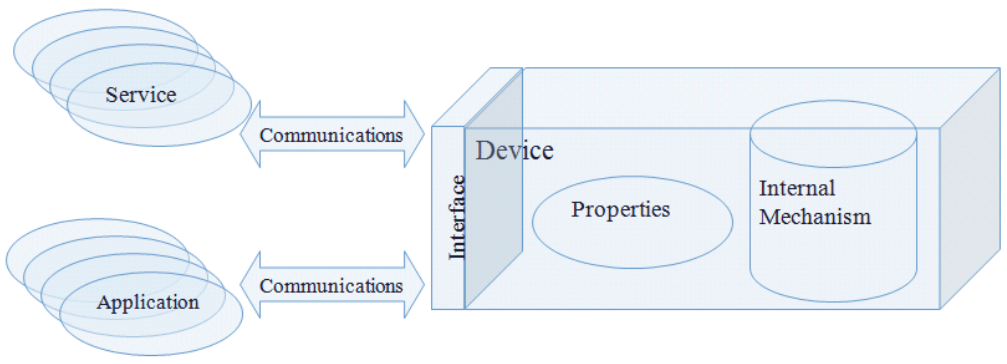
\includegraphics[scale=0.4]{imagens/gatorDDL}
\caption{Caracterização de um dispositivo~\cite{ddlSpec}}
\label{fig:ddlspec}
\end{figure}

Na DDL, um dispositivo é caracterizado como uma entidade com propriedades, mecanismo interno e uma interface, como mostra a figura~\ref{fig:ddlspec}. As propriedades proveem informações a respeito do dispositivo como seu propósito, suas capacidades, seu fabricante e seus requisitos operacionais. Essas informações são críticas para a integração do sistema e para programadores de serviços. O mecanismo interno é responsável pela operação do dispositivo e é desconhecido do mundo externo. A interface do dispositivo é a ponte entre o hiato do mecanismo interno e do mundo externo. Ela especifica a entrada e saída do dispositivo e provê um guia para aplicações e outros serviços interagirem com o aparelho.


Os dispositivos estão classificados em três categorias:
\begin{itemize}
	\item Sensor: apenas provê dados de entrada para o usuário externo.
	\item Atuador: apenas aceita dados de saída do usuário externo.
	\item Dispositivo Complexo: provê dados de entrada e aceita dados de saída do usuário externo.
\end{itemize}

Essa classificação, portanto, se apresenta de forma bastante genérica, pois um dispositivo pode se enquadrar como sensor se limitando a fornecer dados de entrada, como atuador, se limitando a receber dados e tomar ações, ou então será classificado como um dispositivo complexo. Logo a categoria de dispositivo complexo poderá ser utilizada por diferentes tipos de recursos, necessitando conhecer as operações definidas no recurso para, a partir dos seviços providos pelo dispositivo, poder inferir que tipo de recurso é aquele.


\section{Trabalhos Correlatos}
Apresenta-se a seguir alguns projetos de computação ubíqua e como a classificação de recursos é tratada por eles.

\subsection{Gaia}
O \emph{middleware} (Gaia OS) foi criado com o objetivo de dar suporte ao desenvolvimento e execução de aplicações em \emph{Active Spaces}, ambientes com sistemas interativos. Foi projetado para ter uma infraestrutura distribuída que coordena entidades de software e dispositivos heterogêneos em um \emph{smart space}. O Gaia OS expõe serviços para buscar e utilizar recursos presentes no ambiente, ter conhecimento do contexto e provê um \emph{framework} para desenvolver aplicações móveis sensíveis ao contexto, que conheçam os recursos disponíveis, utilizem múltiplos dispositivos e possuam como foco o usuário~\cite{gaia2002}.

\emph{Active Spaces} são espaços físicos como escritórios, salas de conferência, casas, hospitais, campi universitários, cidades, etc, que possuam dispositivos integrados ao ambiente. Tais dispositivos devem prover e obter informações sobre usuários presentes no ambiente, auxiliando-os e/ou facilitando a realizar tarefas que eles não poderiam sem os dispositivos.

\begin{figure}[ht]
\center
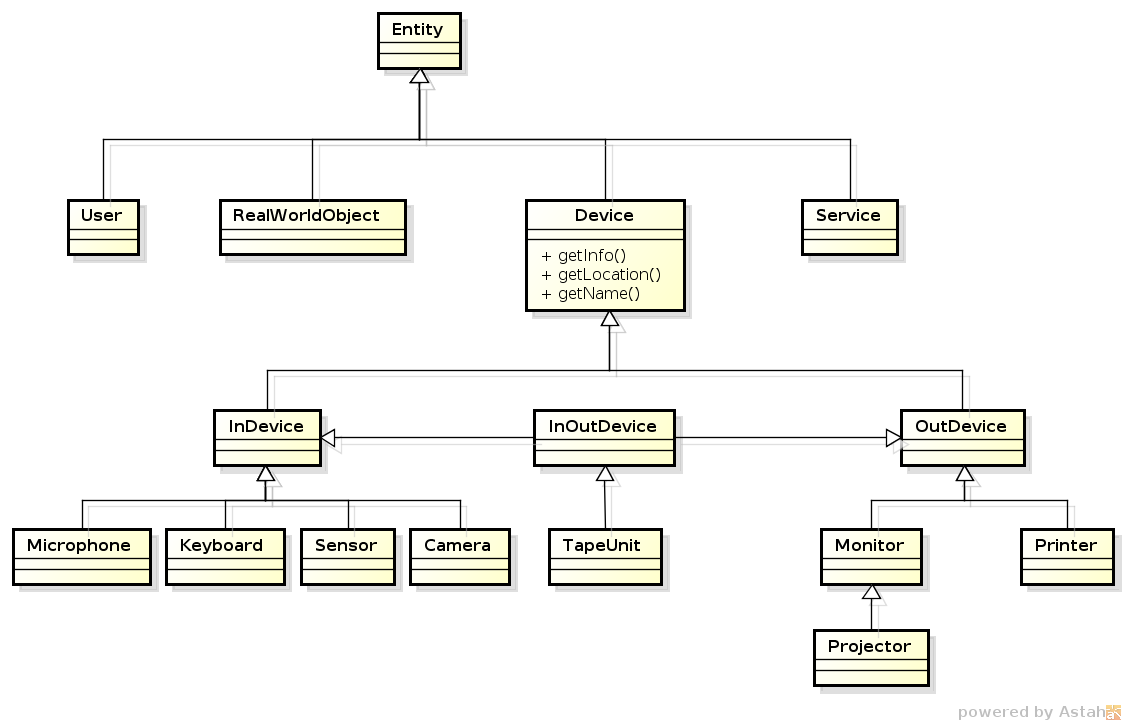
\includegraphics[scale=0.5]{imagens/gaia-devices}
\caption{Diagrama de Classes Simplificado~\cite{gaiaDevices}}
\label{fig:gaiaClassDiagram}
\end{figure}

Desenvolveu-se também um \emph{framework} para a interação entre dispositivos heterogêneos que permite a representação das interfaces dos dispositivos com diferentes níveis de detalhe e especialização. Tais interfaces são definidas utilizando IDL(\emph{Interface Description Language}), que permite a construção de \emph{drivers} de dispositivos em qualquer linguagem de programação garantindo uma facilidade de integração com diferentes dispositivos.

A figura~\ref{fig:gaiaClassDiagram} mostra o diagrama de classes simplificado do projeto. Pode-se observar que a classe \emph{Device} foi especializada em outras classes: \emph{InDevice} e \emph{OutDevice}. Os dispositivos de entrada foram ainda especializados em: \emph{Microphone}, \emph{Keyboard}, \emph{Sensor} e \emph{Camera}, enquanto os dispositivos de saída foram especializados em: \emph{Monitor}, \emph{Printer} e \emph{Projetor}. A interface para dispositivos de entrada e saída foi especializada na classe \emph{Fita}.
\subsection{Amigo}
O projeto Amigo (\emph{Ambient Intelligence for the Networked home environment})~\cite{amigoCore, amigoArch} desenvolveu um \emph{middleware} baseado na \emph{Service Oriented Architecture} (SOA) que integra dinamicamente sistemas heterogêneos para alcançar a interoperabilidade entre serviços e dispositivos. O \emph{middleware} provê a semântica para comunicação e descoberta de dispositivos e serviços disponíveis no ambiente, incluindo dispositivos que utilizam padrões para descoberta, como o UPnP, integrando dispositivos móveis, computadores pessoais, eletrodomésticos e dispositivos de automação residencial.

\begin{figure}[ht]
\center
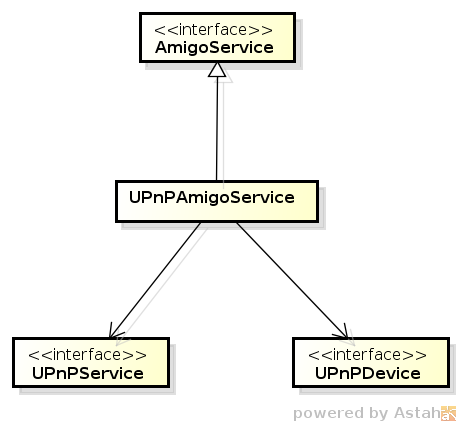
\includegraphics[scale=0.8]{imagens/amigo-interfaces}
\caption{Implementação de um \emph{AmigoService} utilizando serviços UPnP}
\label{fig:amigoInterfaces}
\end{figure}

Além de utilizar o UPnP para a descoberta de dispositivos, o Amigo é compatível com as classificações de dispositivos do UPnP. Quando um dispositivo UPnP é encontrado, é criada uma instância de um \emph{UPnPDevice} e o \emph{driver AmigoUPnP} é notificado e executa o método \emph{getServices} do \emph{UPnPDevice} e cria para cada serviço uma instância do \emph{UPnPAmigoService}. A Figura~\ref{fig:amigoInterfaces} mostra o relacionamento entre as interfaces UPnP com a implementação de uma interface de um serviço do Amigo.

Os serviços do Amigo são modelados em uma Ontologia que é utilizada para comparar serviços e decidir se eles são similares. A classe central da Ontologia é o Componente que representa o dispositivo que provê o serviço. Para representar o que o dispositivo requer e provê, foi introduzido o conceito da Capacidade, dividida em Capacidade Requerida e Capacidade Provida. Uma Capacidade possui parâmetros de entrada e saída que também são modelados em classes. As capacidades são então associadas à Conversas suportadas pelo Componente e relacionadas à mensagens que são empregadas na conversa associada como mostra a Figura~\ref{fig:amigoServiceOntology}.

\begin{figure}[ht]
\center
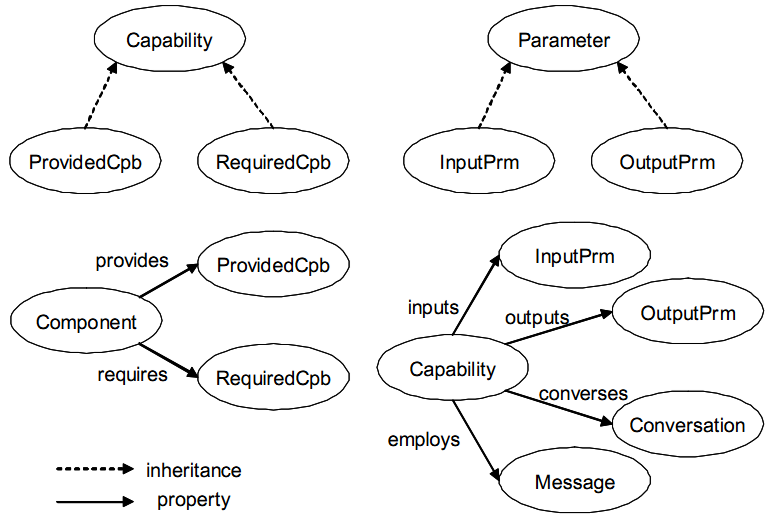
\includegraphics[scale=0.5]{imagens/amigo-ontology}
\caption{Elementos básicos da ontologia de serviços}
\label{fig:amigoServiceOntology}
\end{figure}


\begin{comment}
http://www.hitech-projects.com/euprojects/amigo/publications/IST-004182%20Amigo-IP%20short%20project%20description.pdf
http://www.hitech-projects.com/euprojects/amigo/deliverables/Deliverable%20D1.2-VolII_SOTA_v10_final.pdf
http://www.hitech-projects.com/euprojects/amigo/deliverables/Amigo_WP2_D2.1_v10%20final.pdf
http://www.hitech-projects.com/euprojects/amigo/deliverables/Amigo_WP3_D31b_v1.0.pdf
\end{comment}

\subsection{\emph{Gator Tech}}

O projeto \emph{Gator Tech Smart House}~\cite{gatorTech} tem como objetivo criar ambientes assistivos como casas que terão conhecimentos sobre si e sobre seus residentes criando um mapeamento entre o mundo físico, monitoramento remoto e serviços de intervenção.

Neste projeto foi desenvolvida uma arquitetura para plataforma de sensores orientada à serviços, o Atlas. A plataforma Atlas é uma combinação de nós de \emph{hardware} e \emph{firmware} executado em um \emph{hardware} e um \emph{middleware} executando na rede, que provê serviços em um ambiente. Juntos, esses componentes permitem que qualquer sensor, atuador ou qualquer outro dispositivo sejam integrados e controlados por meio da interface de um determinado dispositivo. Essa abordagem facilita o desenvolvimento de aplicações que utilizam esses dispositivos~\cite{gatorTechLessons}. 

O Atlas é responsável por obter a representação de serviços dos dispositivos conectados e gerenciar os serviços de modo que as aplicações possam obter e utilizar os serviços facilmente. Na implementação do \emph{Gator Tech}, a camada de serviços foi construída sobre o \emph{framework} OSGi que mantém o registro dos serviços de todos os nós conectados. Cada sensor ou atuador é representado no \emph{middleware} Atlas como um pacote de serviços OSGi. 
\subsection{\emph{uOS}}
\label{subsec:introUos}

O \emph{middleware} \emph{uOS} é o resultado do projeto \emph{UbiquitOS} da Universidade de Brasília, cujo foco está na adaptabilidade de serviços. Nesse projeto, os dispositivos presentes em um ambiente inteligente são compostos por recursos que disponibilizam diversos serviços para aplicações ou para o próprio usuário final. Foi concebido um protocolo próprio para comunicação, o \emph{uP (Ubiquitous Protocols)} que utiliza o SLP (\emph{Service Location Protocol}) como técnica para descoberta de dispositivos e \emph{JSON} como formato para troca de mensagens.

\begin{figure}[ht]
	\center
	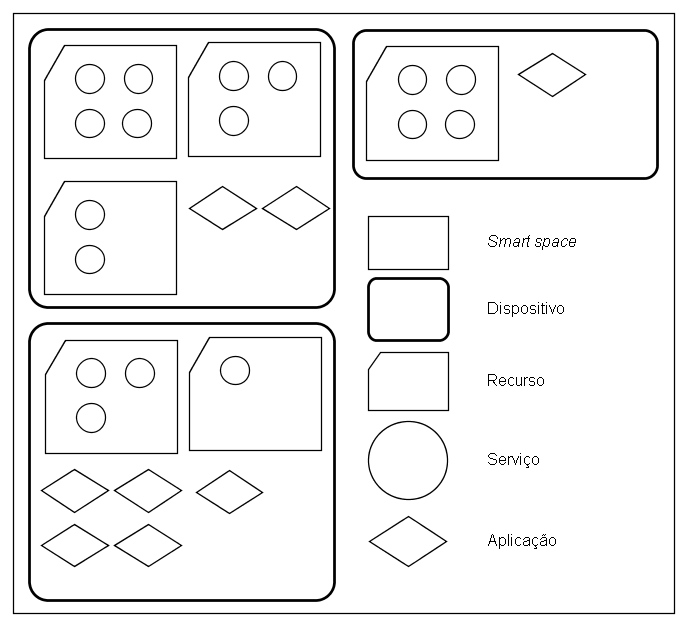
\includegraphics[scale=0.5]{imagens/arquiteturaDSOA}
	\caption{Exemplo da arquitetura DSOA.}
	\label{fig:arquiteturaDSOA}
\end{figure}

O \emph{uOS} utiliza a \emph{DSOA (Device Service Oriented Architecture)}~\cite{buzetoDSOA2010}, uma extensão da \emph{SOA (Service Oriented Architecure)}, como arquitetura. Como mostrado pela Figura~\ref{fig:arquiteturaDSOA}, na DSOA podemos destacar cinco entidades básicas: ambiente inteligente, dispositivo, recurso, serviço e aplicações. O ambiente inteligente é um espaço composto por pelo menos dois dispositivos com capacidade de computação conectados por meio de uma rede de comunicação com os usuários. Um dispositivo é definido como um aparelho com capacidade de comunicação e que pode abrigar aplicações. Um recurso é definido como um grupo de funcionalidades relacionadas que podem ser acessadas por meio de interfaces pré-definidas e é considerada a entidade básica de interação entre dispositivos. Um serviço é a implementação de uma funcionalidade disponibilizada pelo recurso para o ambiente com uma interface conhecida. As aplicações conferem inteligência ao ambiente executando nos dispositivos existentes e, a partir de informações providas pelos recursos conhecidos, podem realizar ações. 

Segundo a DSOA, cada recurso, modelado na forma de um \emph{driver}, é identificado por um nome e não há qualquer tipo de relacionamento entre outros recursos. A \emph{DSOA} não define tipos básicos de recursos.	

\begin{figure}[ht]
	\center
	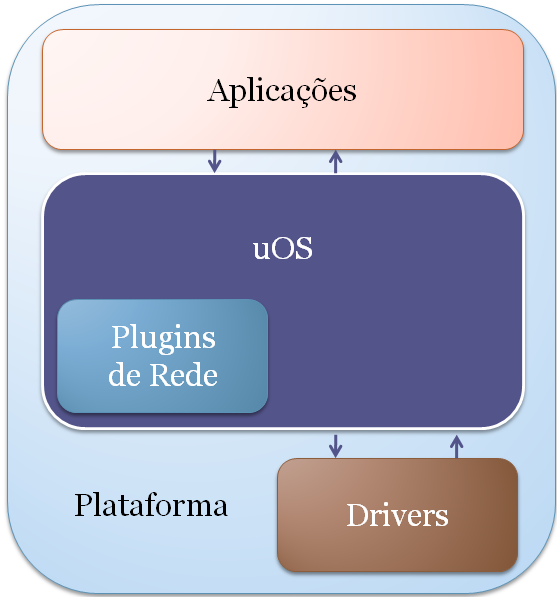
\includegraphics[scale=0.4]{imagens/ecossistemaUbiquitos}
	\caption{Ecossistema do \emph{uOS}.}
	\label{fig:ecossistemaUbiquitos}
\end{figure}

A Figura~\ref{fig:ecossistemaUbiquitos} mostra o ecossistema do \emph{uOS}, em que os \emph{plugins} de rede, abstrações para a rede de comunicação, se destacam como um componente dentro do \emph{uOS}. O \emph{middleware}, por sua vez, utiliza os \emph{plugins} para interfacear a comunicação entre aplicações, por meio dos \emph{drivers}.

\section{Comparativo}
%Apresentar um Comparativo entre as estratégias e conclusões que embasem a definição da proposição de vcs no capítulo seguinte.
A partir da tabela~\ref{tab:comparativo}, pode-se observar que os padrões para a classificação de recursos mostrados neste trabalho são todos estruturados, ou seja, não utilizou-se uma forma dinâmica para representar essa classificação. A maioria dos padrões faz uso de uma classificação relacionada, pois possui a vantagem de aproveitar propriedades já definidas. Além disso, é comum a representação da classificação em arquivos XML, que embora seja um padrão independente de plataforma, tem a desvantagem de possuir uma relevante redundância de dados na sua formatação. Apesar da classificação de alguns padrões possuir a capacidade de ser extensível, é necessário que a nova classe criada pelos fabricantes de um dispositivo passe por uma homologação. Caso do UPnP. O USB possui subclasses derivadas na sua especificação, entretanto não permite novas definições fora do padrão. Em geral, são pouco flexíveis. 

\begin{table}
	\caption{Comparativo dos padrões.}
	\begin{center}
	\resizebox{16cm}{!} {
		\begin{tabular}{ccccccc}
		\hline
							& \textbf{IEEE 1451}	& \textbf{Bluetooth} 	& \textbf{USB}	& \textbf{UPnP} & \textbf{DLNA} & \textbf{DDL}\\
		\hline
		Forma de classificação 		& Relacionada 			& Fixa 					& Relacionada 	& Relacionada 	& Relacionada 	& Fixa \\
		\hline
		Representação 		& IDL 					& Descritor				& Descritor		& XML			& XML 			& XML \\ 
		\hline
		\end{tabular}
	}
	\end{center}
	\label{tab:comparativo}
\end{table}

A tabela mostra ainda uma limitação da DDL (\emph{Device Description Language}), criada para reduzir a complexidade na definição de dispositivos via classes Java, pois, para cada dispositivo que não seja sensor ou atuador, se faz necessária a criação de uma nova classe para esse dispositivo complexo não-relacionada com outras que já tenham sido criadas. Outro fator que impede o uso de subclasses é o fato de na definição do dispositivo estarem definidos também seus serviços, modelados como operações. Se um dispositivo possuir apenas uma operação que receba parâmetros diferentes, por exemplo, a classe anteriormente definida não poderá ser reutilizada. 

\begin{table}
	\caption{Classes presentes nos padrões.}
	\begin{center}
		\begin{tabular}{|ccccc|}
		\hline
									& \textbf{Bluetooth} 	& \textbf{USB}	& \textbf{UPnP} & \textbf{DLNA}	\\
		\hline
		Áudio						& x						& x				& x 			& x				\\
		\hline
		Vídeo						& x						& x				& x				& x				\\
		\hline
		Servidor de mídia			& x						&				& x 			& x				\\
		\hline
		Tocador de mídia			& x						&				& x				& x				\\
		\hline
		Impressora 					& x						& x				& x				& x				\\
		\hline
		Imagem	 					& x						& x				& x				& x				\\
		\hline
		Scanner						& 						& x				& x				& 				\\
		\hline
		Armazenamento				&						& x				& 				& 				\\	
		\hline
		Telefone/PDAs				& x						& x				& x				& x				\\
		\hline
		Teclado						& x						& x				& 				& x				\\
		\hline
		Apontadores					& x						& x				& 				& x 			\\
		\hline
		Interface Humana		 	& x						& x				&  				&  				\\
		\hline
		Específico do fabricante 	& x 					& x				& x				& x				\\
		\hline								
		\end{tabular}
	\end{center}
	\label{tab:comparativoClasses}
\end{table}

A tabela~\ref{tab:comparativoClasses} mostra os principais dispositivos que possuem alguma classe associada nos padrões estudados. O padrão DDL não foi considerado no comparativo de classes devido sua classificação possuir apenas três categorias: sensores, atuadores e dispositivos complexos. Portanto, todos os dispositivos considerados neste comparativo poderiam se encaixar na última categoria. O padrão IEEE 1451 também não foi utilizado no comparativo, pois foi criado para facilitar a comunicação de transdutores, e suas classes não abrangem os dispositivos da tabela.